\suppnote{Supplementary Note S17. Historical fragment assays and local conditional compatibility}\label{si:v4-coherence}
These earlier assays are retained as methodological history and complementary local likelihood evidence. They are superseded as the primary coherence evaluation by the intact-message rubric study in Note S20. Short-fragment similarity and same-prompt substitutions did not establish a suitable measure of ordinary contextual acceptability. This measurement limitation does not prove that the old test was unfair or that actual messages were incoherent.

\suppsubsection{Windows, selection and exclusions}
The original inventory contains 8,280 structural boundaries from 1,440 segmented trials and 240 payloads in four hexadecimal classes. Before scoring, the design adopted the purpose-trained MiniLM encoder\cite{Reimers2019SentenceBERT}, revision \code{c9745ed1d9f207416be6d2e6f8de32d1f16199bf}, with attention-mask mean pooling including nonpadding special tokens, L2 normalization, a 256-token maximum and float32 inference. Model and dependency pins remain in \code{configs/revision_v4/stage2_semantic_encoder.json}. The official source is \url{https://huggingface.co/sentence-transformers/all-MiniLM-L6-v2}.

Mistral's single-space rendering prefix was accounted for before the first pilot, without metric scores. Eligibility changed from 7,113 to 7,133 after the sole right-window amendment. The final 1,147 exclusions have overlapping reasons of 384 actual, 539 ordinary and 238 shuffled boundary-straddling tokens, plus 124 short actual windows. Both sides required three words and exact evaluator alignment. These restrictions do not apply to the intact-message study. Within the selected 3,174 structural boundaries, exclusions are 43/1,058 for Llama, 341/1,058 for Mistral and 40/1,058 for Qwen. The uneven, particularly high Mistral missingness restricts extrapolation beyond eligible windows.

\begin{table}[H]\centering\small
\begin{tabular}{llrrr}\toprule
Generator & Schedule & Structural & Eligible & Excluded \\ \midrule
Llama & Multi-topic & 529 & 507 & 22 \\
Llama & Single-topic & 529 & 508 & 21 \\
Mistral & Multi-topic & 529 & 362 & 167 \\
Mistral & Single-topic & 529 & 355 & 174 \\
Qwen & Multi-topic & 529 & 511 & 18 \\
Qwen & Single-topic & 529 & 507 & 22 \\
\bottomrule\end{tabular}
\caption{Selected structural boundaries before scoring. All models and both schedules are retained for every selected payload. Joint three-arm eligibility removes 424 boundaries, including two trials with no scorable boundary. Detailed artifact-class and overlapping-reason counts remain in the frozen eligibility table.}\label{tab:v4-boundary-eligibility}
\end{table}


Ordinary donors match the exact generator and prompt context, the recipient's forced-stop offset and right length. Selection minimizes prior reuse and breaks ties by a seeded identity hash. Shuffled RankCloak tails use a seeded cyclic order within exact-prompt, schedule and forced-length strata, requiring different payloads and nonidentical right text. Shuffled pilot tails use same-prompt ordinary donors. All source-record hashes, donor payloads and source byte ranges are retained. Right strings are never replaced with a donor from another topic. Exact request caching changes computation counts without dropping repeated inferential units. The final construction audit found no identical complete-window or right-string pair in any of the three full-study arm contrasts.

\suppsubsection{Two control-only pilots}
Both pilots compared ordinary with same-prompt shuffled ordinary windows across all 36 generator, schedule and prompt-category cells. The first used eight left tokens and up to 32 right tokens. The sole predeclared amendment shortened the right cap to 16 and excluded all 69 prior recipient or donor payloads, making the second pilot disjoint in both roles. The ordinary-donor pool retained that exclusion for the subsequent study. The pilots contained 36 and 35 distinct ordinary recipient payload clusters spanning all eight corpus classes. Bootstrap grouping used those recipients, not the encoded identities supplying pseudo-boundary offsets. No window was truncated by MiniLM and no exact-identical right pair remained.

Both semantic intervals in Table~\ref{tab:v4-pilot} cross zero, failing the prospective positive-lower-interval criterion. Context gain passed that specified control-separation check in both pilots. Short fragments and same-prompt overlap limit interpretation of the semantic assay, without identifying the cause of failed separation. No further model or layer search followed. These failures establish neither reader-perceived coherence nor universal incoherence of actual messages.

\begin{table}[H]\centering\small
\begin{tabular}{llrrr}\toprule
Pilot & Metric & Effect & Lower 95\% & Upper 95\% \\ \midrule
Initial & Semantic cosine & 0.0078 & -0.0416 & 0.0572 \\
Initial & Context gain & 2.2200 & 1.7784 & 2.6777 \\
Fresh amended & Semantic cosine & -0.0106 & -0.0728 & 0.0519 \\
Fresh amended & Context gain & 2.0612 & 1.7378 & 2.4109 \\
\bottomrule\end{tabular}
\caption{Blinded ordinary-minus-shuffled ordinary effects. Each pilot uses 36 identities and 2,000 payload-cluster draws. Only context gain has a positive lower interval in both pilots. Semantic validation remains unsupported.}\label{tab:v4-pilot}
\end{table}


\suppsubsection{Fixed-path conditional compatibility}
The historical ordinary controls use temperature 0.8 and top-\(p\) 0.95 sampling, whereas RankCloak tails are greedy. The contrast includes this continuation-policy difference.

The complementary metric uses the existing evaluator map, Llama text scored by Qwen, Qwen by Mistral and Mistral by Llama. For the same evaluator tail-token path \(y_{1:n}\), it measures
\begin{equation}
G=\frac{1}{n}\sum_{i=1}^{n}\left[\log p_E(y_i\mid P,L,y_{<i})-\log p_E(y_i\mid P,y_{<i})\right],
\label{eq:v4-context-gain}
\end{equation}
where \(P\) is the evaluator-tokenized rendered prompt, including its declared BOS policy, and \(L\) is the evaluator-token prefix of the joint visible left/right window. The sequence \(y_{1:n}\) is the remaining suffix of that joint tokenization. Both contexts append these exact target IDs and share denominator \(n\). The prompt-only pass reuses these tail IDs even if standalone tail tokenization differs. Raw mean conditional tail log likelihood is retained as a secondary measure. This is a fixed-token-path contrast, not the difference between independently tokenized string likelihoods. Whole-message likelihood is not substituted for a boundary measure.

Exact byte alignment excludes boundary-straddling tokens. A batched LM route failed the fixed-fixture numerical tolerance for each evaluator, so scoring retained serial batch and microbatch size one. Embedding batching passed its separate fixture. No unvalidated KV reuse was introduced.

Actual minus ordinary context gain was 0.1575 nats per tail token (95\% interval [0.1098, 0.2066]), and actual minus shuffled gain was 2.3265 [2.2705, 2.3912]. The secondary raw conditional-likelihood contrast was 0.0619 [0.0277, 0.0981]. Generator-specific raw conditional intervals include zero for Mistral and Qwen. These local findings establish neither semantic coherence nor a causal payload-boundary effect.

\begin{table}[H]\centering\small
\begin{tabular}{lrrr}\toprule
Contrast & Difference & Lower 95\% & Upper 95\% \\ \midrule
actual minus ordinary & 0.1575 & 0.1098 & 0.2066 \\
actual minus shuffled & 2.3265 & 2.2705 & 2.3912 \\
ordinary minus shuffled & 2.1690 & 2.1185 & 2.2215 \\
\bottomrule\end{tabular}
\caption{Exploratory paired context-gain differences in nats per evaluator tail token for the completed frozen sample. Segments are averaged within trials and trials within payloads. Intervals use 2,000 payload-cluster draws within artifact class and condition on the fixed donor corpus.}\label{tab:v4-coherence}
\end{table}

The measured-cost admission selected 92 of 240 payloads, with 23 per class, preserving all models and schedules. The selected structural inventory contains 3,174 boundaries in 552 trials. The completed analysis contains 2,750 eligible boundaries, 8,250 arm-specific units and 550 trials. Every planned request completed. Selection used no RankCloak metric scores. The sample supports the reported precision only, not a guaranteed effect or a claim about excluded boundaries.

\begin{figure}[H]\centering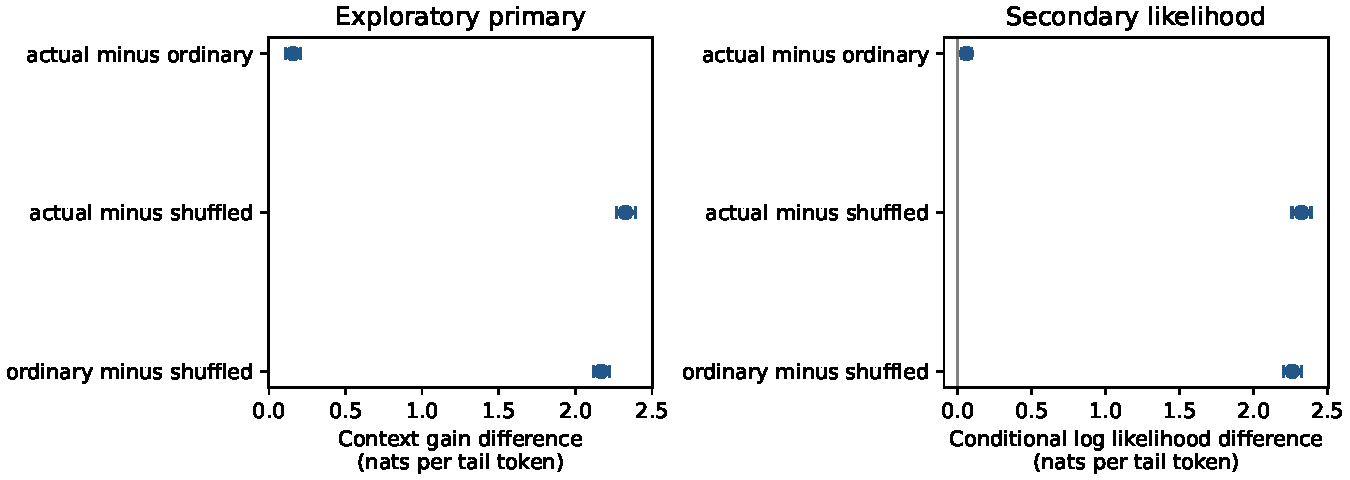
\includegraphics[width=\textwidth]{figures/v4_boundary_coherence.pdf}\caption{Paired boundary metric differences with payload-cluster 95\% intervals. Context gain passed the specified pilot control-separation check and is used here exploratorily. Raw conditional likelihood is secondary. These automated results do not establish perceived naturalness.}\label{fig:v4-coherence}\end{figure}

\begin{table}[H]\centering\small
\begin{tabular}{llrr}\toprule
Generator & Contrast & Context gain [95\% interval] & Conditional [95\% interval] \\ \midrule
Llama & actual minus ordinary & 0.2632 [0.1717, 0.3502] & 0.1716 [0.1025, 0.2428] \\
Llama & actual minus shuffled & 2.3903 [2.2945, 2.4883] & 2.4070 [2.3204, 2.5007] \\
Qwen & actual minus ordinary & 0.0978 [0.0272, 0.1656] & 0.0322 [-0.0184, 0.0863] \\
Qwen & actual minus shuffled & 2.1414 [2.0641, 2.2182] & 2.1893 [2.1063, 2.2703] \\
Mistral & actual minus ordinary & 0.1076 [0.0098, 0.2112] & -0.0089 [-0.0840, 0.0682] \\
Mistral & actual minus shuffled & 2.4493 [2.3234, 2.5903] & 2.3865 [2.2536, 2.5292] \\
\bottomrule\end{tabular}
\caption{Generator-specific paired effects under the fixed cross-family evaluator map. Values are in nats per evaluator tail token. Context gain is exploratory and raw conditional likelihood is secondary. Each interval uses the same 2,000 stratified payload draws as the pooled analysis. The evaluator and tokenization vary with generator, limiting interpretation of differences across rows.}\label{tab:v4-coherence-models}
\end{table}


The ordinary arm uses 411 donor payloads across 2398 source identities. Maximum donor-payload reuse is 18 and maximum source-identity reuse is 2.

The shuffled arm uses 240 donor payloads across 2354 source identities. Maximum donor-payload reuse is 32 and maximum source-identity reuse is 4.

For actual minus ordinary, deleting each reference donor payload in turn gives point estimates from 0.1504 to 0.1643. This is a donor-influence diagnostic, not a population interval incorporating two-way donor sampling.

For actual minus shuffled, deleting each reference donor payload in turn gives point estimates from 2.3210 to 2.3363. This is a donor-influence diagnostic, not a population interval incorporating two-way donor sampling.

All scored windows have eight generator tokens on the left and eight to sixteen on the right. These short contexts limit interpretation beyond local transitions.

Standalone tail tokenization differed from the retained joint-tail path in 3057 units. The conditional and reference passes nevertheless scored the same IDs and denominator for each comparison. All exact source mappings and per-model effects remain in the joined tables.

\suppsubsection{Predeclared illustrative boundaries}

The weak, typical and strong examples use the minimum, upper-middle and maximum actual context gains, with identity-hash tie breaks. The marker shows the exact boundary. Literal newline markers retain formatting.

\noindent\begin{minipage}{\linewidth}

\paragraph{Weak context gain.}

The score is -0.2986 nats per tail token. Both windows use the following source.

\begin{flushleft}\small Source \code{revision_v1_primary_v2_payload_fidelity_v2__60c7c024bb462f543873__segment_1}\\ Evaluator \code{qwen2_5_7b_instruct_q4_k_m}.\end{flushleft}

Left source bytes are [0, 22). Right source bytes are [22, 104).

\begin{quote}\small **)\textbackslash{}nHere's how I came:\textbf{ [BOUNDARY] } I was walking by your garden yesterday and noticed how beautiful the flowers are!\end{quote}

\end{minipage}\par\medskip

\noindent\begin{minipage}{\linewidth}

\paragraph{Typical context gain.}

The score is 1.8772 nats per tail token. Both windows use the following source.

\begin{flushleft}\small Source \code{revision_v1_primary_v2_payload_fidelity_v2__339ba03e74127c1632ff__segment_0}\\ Evaluator \code{mistral_7b_instruct_v0_3_q4_k_m}.\end{flushleft}

Left source bytes are [0, 32). Right source bytes are [32, 59).

\begin{quote}\small  \textbackslash{}n\textbackslash{}nEmail:\textbackslash{}nRecieved Date \& Client\textbf{ [BOUNDARY] } Name: 2023-10-15, ABC Corp\end{quote}

\end{minipage}\par\medskip

\noindent\begin{minipage}{\linewidth}

\paragraph{Strong context gain.}

The score is 7.7527 nats per tail token. Both windows use the following source.

\begin{flushleft}\small Source \code{revision_v1_primary_v2_payload_fidelity_v2__5cb9b4336f971271f1d1__segment_1}\\ Evaluator \code{llama3_8b_instruct_q4_k_m}.\end{flushleft}

Left source bytes are [0, 31). Right source bytes are [31, 52).

\begin{quote}\small  Be creative; don\textbackslash{}'d worry over\textbf{ [BOUNDARY] }much about grammar.\textbackslash{}n\textbackslash{}n\end{quote}

\end{minipage}\par\medskip

The highest context-gain example contains the word-internal join \code{over[BOUNDARY]much} and retains malformed wording. The labels refer only to the predeclared metric ordering. They are not ratings of grammaticality or meaning.


\suppnote{Supplementary Note S18. Transport decomposition and fixed-message decoding}\label{si:v4-transport}
The historical composite Markdown operation normalizes CRLF and CR to LF, strips outer whitespace, trims each line's trailing whitespace, and inserts \code{> } before each line. A receiver then retokenizes the whole string and applies the original saved token offsets. Thus prefix-induced span misalignment, changed token boundaries and changed contextual ranks are separate possible mechanisms. Whitespace removal can be irreversible. The tested operation does not represent every Markdown editor or transfer workflow. The isolated line-ending arm normalizes CRLF and CR to LF, matching this component of the composite operation. The historical LF-to-CRLF result remains a separate condition.

The five diagnostic sources are selected by SHA256 of seed and identity within model and executed unchanged-visible-text recovery status. The historical raw unmodified rows are retained as saved-ID references. To avoid relabeling these as executed visible-text trials, the baseline uses actual historical transformation rows with identical source and observed bytes in every segment. These are identified by work ID in the retained source table. Mistral has no eligible successful visible baseline. We preserve the original composite outcomes and decode only missing distinct model-input requests for the five decompositions.

Twenty-five logical cover arms contain 135 constituent segments. Exact input matching reuses 53 historical segment requests and leaves 26 new distinct segment replays. Their preflight counts are 9 Llama, 4 Mistral and 13 Qwen, giving a preflight upper count of 805 context and received tokens before early rejection. Historical replays allocated 4,096 context positions, whereas the bounded worker allocates 512. All 53 reused inputs were subsequently checked at the new capacity and reproduced their historical ranks and errors exactly. These checks evaluated 1,626 tokens and add no logical cover arms. In total, 79 distinct segment inputs were executed within the same 25 arms. Agreement is demonstrated for these short inputs, not for arbitrary context-capacity changes. All 27 prefix-only segment instances change token zero and present a prohibited first forced token. The safe-text mask rejects that token, so these particular failures terminate before a rank sequence is returned. Later contextual-rank changes are not measured in those rejected segments. Prefix-only covers therefore all fail. Outer trimming and wrapper removal each recover the same originally failing Mistral case, while trailing trimming retains the selected Qwen success. This nonmonotonic behavior is why a small mechanism diagnostic cannot estimate a general recovery rate or justify claiming all Markdown workflows fail.

\begin{table}[H]\centering\small
\begin{tabular}{lrrrrrrr}\toprule
Case & Visible & Composite & Prefix & Outer & Trailing & LF & Unwrap \\ \midrule
Llama failure & 0 & 0 & 0 & 0 & 0 & 0 & 0 \\
Mistral failure & 0 & 0 & 0 & 1 & 0 & 0 & 1 \\
Qwen failure & 0 & 0 & 0 & 0 & 0 & 0 & 0 \\
Qwen success & 1 & 0 & 0 & 0 & 1 & 1 & 0 \\
Llama success & 1 & 0 & 0 & 0 & 0 & 1 & 0 \\
\bottomrule\end{tabular}
\caption{Illustrative exact byte recovery. One denotes success and zero failure. Visible baselines are executed historical transformations that left every source byte unchanged. The historical unmodified reference itself aliases saved-ID recovery. The five decompositions use saved offsets and no payload-informed repair. Mistral has no eligible successful visible baseline. These cases do not estimate population rates.}\label{tab:v4-transport}
\end{table}


The machine-readable segment diagnostics retain changed byte ranges, source and observed token IDs, saved start/stop offsets, the extracted forced span, recovered ranks, first differing or missing rank position, explicit filter/replay errors and recovered payload bytes. A prohibited received token can cause immediate filter rejection, so a missing rank is not reported as a measured rank value. Declared wrapper removal only removes the prefix from every transported line. It neither uses the source payload nor searches offsets. It does not restore whitespace already removed by the composite operation.

\suppsubsection{Directional cross-quantization endpoint}\label{si:v4-fixed-quant}
The shared-history audit reconciles 1,920 pairs and 244,440 positions. Encoded messages contribute 960 pairs, 122,220 positions and 56,321 observed-rank changes. Ordinary controls contribute 960 pairs, 122,220 positions and 13,207 changes. These pooled counts differ from an average of per-message change fractions and should not be substituted for the historical mean fraction 0.4639.

The new offline endpoint applies original bounded-codec metadata to saved Q8 ranks on the historical Q4 received-token path and compares actual bytes. All 960 encoded rows are supported and none recovers the original payload. For B8, 471 of 480 trials contain invalid ranks, totaling 3,587 invalid positions. For B16, 295 of 480 contain invalid ranks, totaling 904 positions. The other 194 trials decode accepted but incorrect byte strings. Accepted means that bounded ranks and length are valid under the retained decoder, which discards the declared terminal padding without checking its value. One of these accepted wrong reconstructions has nonzero discarded padding. It is not an integrity check. Ordinary controls have no payload endpoint. This result neither reruns generation nor estimates Q8-to-Q4 decoding. Within-quantization saved-ID recovery and bidirectional detector transfer remain separate results.

\suppnote{Supplementary Note S19. Configuration, rank margins and computational cost}\label{si:v4-theory}
\suppsubsection{Compatibility and conditional recovery}
The canonical fingerprint demonstration records all eleven contract components and rejects an intentional quantization mismatch. Every component has a mismatch test and serialization is deterministic under reordered input keys. These checks protect declared compatibility only. They do not authenticate a header or guarantee identical transport, nor were headers added to the original protocol.

For a declared ensemble, let \(p_t\) be the conditional probability of rank disagreement at position \(t\), given agreement at all preceding positions. Complete rank agreement has probability \(\prod_t(1-p_t)\). This identity does not infer the probabilities from a model version label. Byte recovery additionally requires valid framing and codec inversion. Tokenizer changes may split or merge tokens and shift saved offsets, whereas gate disagreements alter which positions consume payload digits.

\suppsubsection{Quantization margin and received-token history}
For a fixed received history, allowed set and tie rule, suppose every logit changes by at most \(\epsilon\). Then a pair separated by more than \(2\epsilon\) cannot reverse order. Protecting an observed token's rank requires that no candidate crosses it. Strictly separated immediate upper and lower neighbors suffice when the bound holds for all candidates. Ties and smaller gaps lack that guarantee. This is a sufficient mathematical condition, not an observed maximum quantization error. The retained evidence does not contain all neighboring logits and no quantitative margin distribution is claimed.

Independent generation can choose a different next token and then condition on a different history. Observed-token replay always feeds the received cover tokens, not recovered payload symbols, back into its model. Incorrect payload digits alone therefore do not cause the same cover-history feedback. Tokenization changes, span shifts and gate disagreements require separate synchronization arguments.

\suppsubsection{Trace-informed detection and proposed fallback}
The evaluated model-aware detector consumes saved untempered full-vocabulary token log probabilities. Reproducing them requires the model and numerical backend, original token IDs, prompts, boundaries and reset schedule. Visible-text retokenization is a distinct, unvalidated access condition. Ordinary sampling instead uses temperature 0.8 and top-\(p\) 0.95. Payload rank choices need not follow that distribution, and bounded ranks do not enforce distribution matching. Temporal structure and serialized digits are plausible additional cues, not established causal contributions. A sequence-KL decomposition needs its support and integrability assumptions. In particular, a top-\(p\) reference can assign zero mass to a forced token. AUC cannot be converted into KL. An observer with the full receiver configuration may decode.

The proposed fallback identifies a supported configuration, frames independent blocks with explicit context resets and integrity checks, and applies bounded outer error/erasure correction before requesting retransmission. For a conventional code of minimum distance \(d\), unique correction is guaranteed when \(2e+s<d\) for \(e\) errors and \(s\) located erasures under its channel assumptions. ECC cannot reconstruct an arbitrary wrong model codebook or repair persistent synchronization loss. Repeating a transmission under the same unresolved mismatch does not solve it. Metadata, redundancy, checks and retries consume length and compute and can introduce detector cues. This is an unimplemented proposal, not a recovery result.

\suppsubsection{Model work and coding operations}
Let \(M=\sum_j F(P_j)+\sum_t D(h_t)\) collect prompt-prefill and incremental model work at the actual context lengths. Let \(b\) denote arithmetic precision, \(K\) retained arithmetic candidates and \(n_l\) group sizes on an ADG recursion path. Table~\ref{tab:v4-complexity} gives non-model operation counts derived from the inspected code or primary pseudocode. It does not normalize different implementations' hardware or kernels.

\begin{table}[H]\centering\small
\begin{tabularx}{\textwidth}{L{0.20\textwidth}Y}
\toprule
Procedure & Non-model work and qualifications \\
\midrule
RankCloak selection & \(O(V+A\log A)\) per call. Full sorting is used even for rank one. Diagnostic and rank-\(B\) calls can repeat the sort. \\
Known-token recovery & \(O(V+A)\) per call by greater-score and lower-ID tie counting. Added log-probability and entropy diagnostics require vocabulary passes. \\
Arithmetic coding & The inspected implementation sorts the full vocabulary before truncation, rounds cumulative intervals and scans candidates, giving \(O(V\log V+V+K+b)\) per step at fixed precision. Optional tokenization repair adds data-dependent work. \\
SAAC & Full sorting and a cumulative mass scan precede adaptive truncation. The inspected route has \(O(V\log V+V+K+b)\) per step, with adaptive \(K\) and finite-precision updates. \\
ADG grouping & Sorting and nearest-probability binary searches recur within selected groups. Efficient ordered deletion and maintained sums permit \(O(\sum_l n_l\log n_l)\). Literal list deletion or repeated sums can add \(O(\sum_l n_l^2)\). Decoding reconstructs the same grouping. \\
\bottomrule
\end{tabularx}
\caption{Implementation-specific operation counts in addition to model work \(M\). Arithmetic and SAAC source revisions and hashes are archived with primary-source links. ADG is assessed from Algorithm 1 and its selected-group recursion\cite{Ziegler2019NeuralLinguisticSteganography,Shen2020SelfAdjustingArithmetic,Zhang2021ProvablySecureGenerative}.}\label{tab:v4-complexity}
\end{table}

For \(m\) serialized bytes, B8 consumes \(\lceil8m/3\rceil\) ranks and B16 consumes \(2m\). Hex-nibble consumes one rank per displayed character. Direct-subword rank measurement and inversion require additional payload-side model passes. Gate skips, lead-ins and tails increase emitted positions without increasing payload ranks, while segmentation repeats prefills. Peak memory includes weights, KV state, \(O(V)\) temporaries and \(O(CV)\) stored scores for configured context limit \(C\) when \code{logits_all=True}. Scalar saved traces require \(O(T)\) storage. Sequential segments reuse peak buffers. Host transfers, kernels, serial scheduling and diagnostic constants prevent a wall-time ranking from these asymptotic expressions.
